\documentclass{article}
\usepackage[utf8]{inputenc}
\usepackage[margin=1in]{geometry}
\usepackage{amsmath}
\usepackage{amsfonts}
\usepackage{graphicx}
\usepackage{graphics}

\title{The Number Theory and Application of Pythagorean Triples}
\author{Trevor Farrell}
\date{March 2022}

\begin{document}

\maketitle

\section{Diophantine Equations – A Summarized History}

For basically as long as humans have been humans, we’ve held an obsession with the natural numbers. Being that they’re the ones that come the most organically to us, it should come as no surprise that we’ve even gone out of our way to name and label a whole selection of multi-variable equations with the potential for easy, comprehensible integer solutions. Euclid’s proof of the Pythagorean theorem around 300 BC \cite{historyofmathematics} has proven to be one such gratifying means of attaining a series of exponential Diophantine solutions, uncovered early on in our mathematical history. History has yet to record the first definitive instance where (and when) somebody discovered the uncanny and entirely convenient assemblage made from three-four-five triangles. Since that time our thirst for straightforward solutions to these such problems have only grown. \\

A fine place to begin our journey may yet start with Diophantus (c. 200/214 AD – c. 284/298 AD) one of the earliest recorded mathematicians whose studies specialized in approaching such problems, and for which the category of problem is named after. His findings are best cataloged in his magnum opus collection of books titled Arithmetica, which were fortunately -- for reasons soon to be made apparent -- translated from Greek to Arabic by Qusta ibn Luqa (820–912) during the Islamic Golden Age. Although the majority of his surviving work directs its focus towards solutions to quadratic equations, the immediate application of the approaches outlined were invaluable. Diaphantus described various categories of linearly independent numbers, described as 'linear number, plane number, solid number', and while he hinted at inequalities for larger order Diophantine equations (e.g., Fermat's Little Theorem) he never addressed them directly. While Diophantus laid the groundwork for arithmetic, it would be his successors in other lands who would apply algeberic reasoning to his studies.  \\

\section{Al-Khazin's Number Theory}

Fast forwarding through time to the Islamic Golden Age, we find ourselves analyzing the works of al-Khazin, (c. 900–971) a mathematician  (although some scholars argue he may have been two mathematicians) who focused principally in astronomy. Although his flawed geocentric model of the solar system – one consisting of an off-center orbiting sun – may lead some historians to consider him a third-rate mathematician, al-Khazin’s advances in number theory are of indisputable significance. Outlined in full, and with no shortage of rigor, al-Khazin advanced the study of pythagorean triples by procuring a definitive means of generating Primitive Pythagorean Triples, or PPTs; that is to say, triples that are not simple multiples of pre-established triples. His method is illustrated below:\\

\newpage

\textbf{Lemma 1:} There exists no couple of odd square integers whose sum is also a square. \\

\textbf{Proof:} Let's make some assumptions to the contrary. Let $\alpha, \beta$ be square odd integers -- that is, let $a = \alpha ^2 \ , \ b = \beta^2 \ , \ a,b \in 2n+1 \ , \ n \in \mathbb{N} $ -- such that $\alpha + \beta = \gamma $ where $\gamma$ is a square, that is, $c = \gamma^2 $. From this, let's say $a^2 + b^2 = c^2$.\\

Since $\alpha, \beta$ are odd, $\gamma$ \textit{must also} be odd; for the same reason, \textit{a,b} must be odd, as they're both odd numbers multiplied by odd numbers. Since an odd number subtracted from an odd number is an even number, we know $b-c$ is even. furthermore, 

$$ a^2 = c^2 - b^2 = (c+b)(c-b) = (c-b)^2 - 2b(c-b) $$

However, take note that an even minus an odd is odd, so $(c-b)$ must be odd, given our initial assumptions. Also, noting that

$$ a^2 = [a+(c-b)][a-(c-b)]+(c-b)^2 $$

we may deduce

$$ 2b( c-b ) = [ a + (c-b) ][a - (c-b)] $$ 

Given that $a+(c-b)$ is even, as is $(a-(c-b))$, then our second number should be divisible by four, while our first number is odd -- this is an absurdity and a contradiction. And so we understand that no matter how hard we try, we cannot expect a square to be made from the sum of two odd squares -- at \textit{least} one must be even. \\

\textbf{Lemma 2:} For a triangle with sides $\alpha,\beta$ where $\alpha,\beta$ are binomial even numbers, i.e, $\alpha,\beta, \in 2^n \ , \ n \in \mathbb{N}$, then the value of our hypotenuse \textit{cannot} be binomial even number. \\

\textbf{Proof:} Assume $a=2^m \ , \ b=2^n$ where $m,n$ are integer numbers \textit{and} where $m<n$. This would guarantee that $\frac{a}{b} = \frac{2^m}{2^n} = 2^{-(n-m)}$. Additionally, 

$$ \frac{a^2}{a^2 + b^2} = \frac{1}{1+2^{-2(n-m)}} $$

However, this equality doesn't make any sense, since it'd be implying $a^2 + b^2 = \frac{1}{1+2^{-2(n-m)}}$ is a square, which is impossible -- squares are never consecutive. Another absurd contradiction is added to the tally.\\

\textbf{Lemma 3:} For reasons that will be made clearly in a minute, consider the following:

$$ (a+b)^2 = b^2 + 4 \frac{a}{2} \Big( b+ \frac{a}{2} \Big) $$

where $a$ is even and $b$ is odd. This is actually a fairly straightforward identity, which al-Khazin borrows liberally from Euclid, via proposition II-8 of \textit{Elements}. With all of this lain out on the table, what do we have at our disposal? It is here that al-Khazin shows his genius; by using these Lemmas synthesized in a single proposition, he demonstrates a rigorous means of generating Primitive Pythagorean Triples: \\

\textbf{Proposition:} Suppose we have some numbers $a,b$ such that $a$ is even and $b$ is odd, and such that $a^2 + b^2 = c^2$. Note:

$$ c = \Big( b + \frac{c-b}{2} + \frac{c-b}{2} \Big) $$

By Lemma 3, 

$$ c^2 = b^2 + 4 \Big( b - \frac{c-b}{2} \Big)*\frac{c-b}{2} $$

and since $a^2 + b^2 = c^2$, we have an identity for $a^2$:

$$ a^2 = 4 \Big( b - \frac{c-b}{2} \Big)*\frac{c-b}{2} $$

Close attention is warranted here: since our value to the right side of the equality is a square, we do well to remind ourselves that -- being the product of two values -- that its second-term reciprocal is also a square. Al-Khazin implores us to consider for a moment this object, represented in relationship with $p,q$, as follows:

$$ \frac{4 \Big( b - \frac{c-b}{2} \Big)}{\frac{c-b}{2}}  = \frac{p^2}{q^2} $$

where $p,q$ have at best a greatest common divisor of one, and where $(p >q)$. \\

With this being the case, $p$ and $q$ have innately unique parity, and we may generate unique primitive triples with the following:

$$ b = p^2 - q^2 \ , \ a = 2pq \ ,\ c = p^2 + q^2 $$

Setting aside the obvious good humor that comes from the spirit of Diophantus emerging in the form of what resembles quadratic coefficients, al-Khazin was also quick to emphasize the significance of the surjective relationship between $(p,q) \longrightarrow (a,b,c)$. \cite{Rashed} Although doing as much helps to reassure the reader that the sequential solutions for Pythagorean Triples are indeed primitive, the application need not stop there; let us fast forward through time a few more centuries to see just how such a unique relation serves a purpose in the age of computation. \\

\section{Modern Cryptography}

Al-Khazin's advancement holds indisputable significance in the field of number theory, with no shortage of attention paid in the modern day towards its potential for cryptography. For each of the triples generated by his method, for any one ordinary pair of Pythagorean numbers – ones with no common divisor – there can exist at most one integer solution. And by its surjective nature, our primitive Pythagorean triples are appealing to security analysts and cryptographers as a means of constructing one-way functions. \\

However, the fun need not stop there: by using a New Pythagorean Triple algorithm formula derived by Newton, \cite{dataencryption} this definition can be re-stated to the following: for any numbers $p$ and $q$ (again, one of them odd and the other even) there are at least two fundamental solutions $(a_1,b_1,c_1)$ and $ (a_2,b_2,c_2) $ -- in some special circumstances, there may even exist some unique third solution $(a_3,b_3,c_3)$. \cite{pythagoreancrypto} Newton's method isn't wholly daunting -- since each of the faces for our Pythagorean figure may be treated as a square, the results of our previous generation may be reiterated: 

$$ (p^2-q^2)^2 +(2pq)^2 \cong (p^2+q^2)^2 $$

otherwise written as

$$ x = d(p^2 - q^2) \ , \ y = 2dxy \ , \  z = d(p^2 + q^2) \ , \ d = (x,y,z) $$

Where $d=1$ signifies a primitive nature. Since the square of each solution now allows for the potential of negative numbers, we find ourselves stepping outside the confines of the previous solutions. Working through the system and isolating our variables, we discover a new piecewise representation for our variables: 


\begin{equation*}
 (a,b,c) = \left\{
        \begin{array}{ll}
            x = 2p^2 \mp 2pq \\
            y = q^2 \mp 2pq \\
            z = 2p^2 \mp q^2 \mp 2pq \\
        \end{array}
    \right.
\end{equation*}

With three possible solutions available to us, we can illustrate the framework necessary for establishing a symmetric cryptosystem. Consider following hand-selected values employed for a cryptosystem, where $k$ is our private key, $m$ is our secret message, and $c$ is our encrypted text:

\begin{center}
    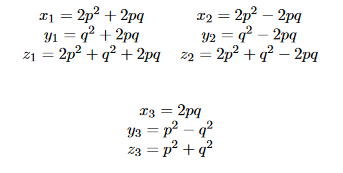
\includegraphics[scale=0.75]{cryptography_latex.PNG}

\end{center}

Where our private key takes on the following form:

$$ (x_1, y_1, z_1), (x_2, y_2, z_2), (x_3, y_3, z_3)(mod26)$$

Where $c = m + k(mod26)$ serves to encrypt our message, and where $m = c - k(mod26)$ serves to decrypt our message. Since our values are selected to have no common divisors, there would exist no known method for decrypting our cyphertext better than sequential guessing. And provided we used a sufficiently large numbers for our key generation, even guessing may prove insufficient -- after some point, the likelihood of 'decrypting' a coherent message from the assembly that does \textit{not} match the original plaintext (akin to the library of babel) becomes every bit as likely as the chances of uncovering the original intented message. \\

Perhaps the most impressive aspect of this cryptosystem is the lineage behind it. Sprouting from fundamentals in human curiosity in pre-biblical times, and passing through the hands of big-name mathematicians across multiple continents and languages, the results continue to find relevance in the modern era. Through Euclid, Diaphantus, Pythagorus, Al-Khazin, Newton, and on to those who study mathematics to this very day, the number theory of those who dared to speculate about the relationship between integers on the sides of a given triangle has firmly cemented itself as immortal. 

\newpage
\bibliographystyle{plain}
\bibliography{bibliography.bib}

\end{document}
